\documentclass[border=7pt]{standalone}
\usepackage{tikz}
\usepackage{tikz-3dplot}
\usepackage{pgfplots}
\usepackage{graphics}
\pgfplotsset{compat=1.13} 

\begin{document}


%%%%%%%%%%%%%%%%%%%%%%%%%%%%%%%%%%%%%%%%%%%%%%%%%%%%%%%%%%%%%%%%%%%%%%%%%%%%%
%%%%%%%%%%%%%%%%%%%%%%%%%%%%%%%%%%%%%%%%%%%%%%%%%%%%%%%%%%%%%%%%%%%%%%%%%%%%%
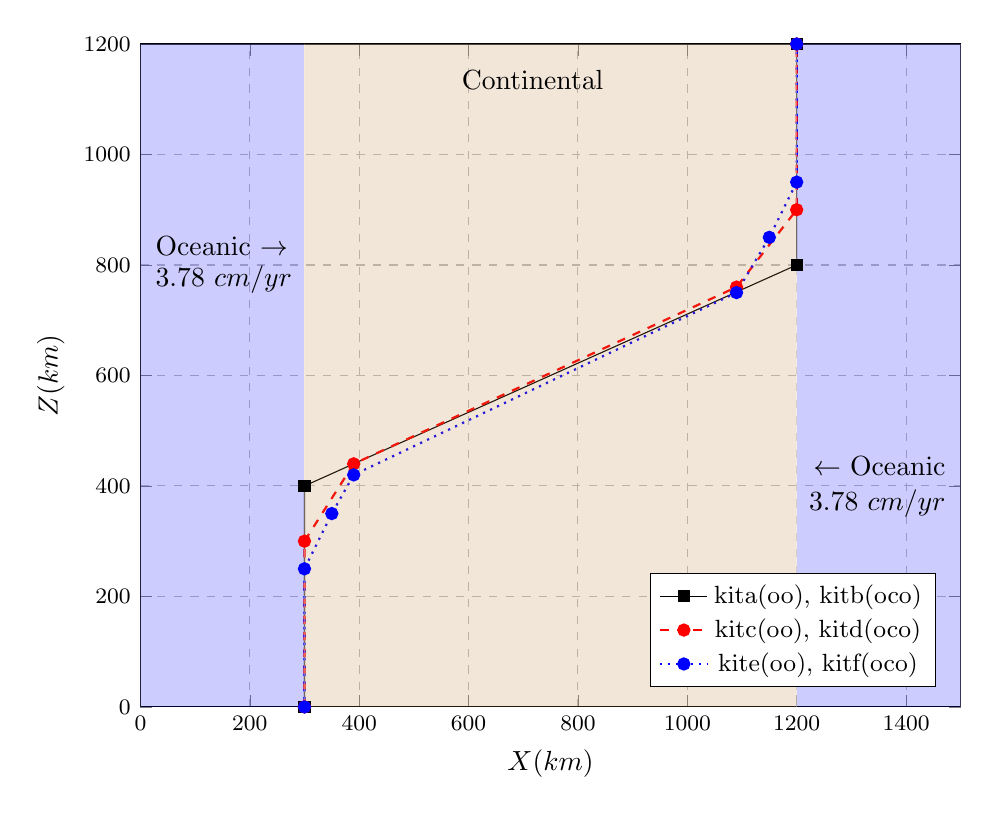
\begin{tikzpicture}

%%%%%%%%%%%%%%%%%%%%%%%%%%% Axes Set-up %%%%%%%%%%%%%%%%%%%%%%%%%%%%%%%
\begin{axis}[ylabel=$Z (km)$,xlabel=$X (km)$,
width=12cm,height=10cm,
xmin=0,xmax=1500,
ymin=0,ymax=1200,
ymajorgrids=true,
xmajorgrids=true,
grid style=dashed,
tick label style={font=\footnotesize},
legend style={font=\small},
/pgf/number format/.cd, 
set thousands separator={},
legend pos=south east]

%%%%%%%%%%%%%%%%%%%%%%%%%%% Plot 1 %%%%%%%%%%%%%%%%%%%%%%%%%%%%%%%
\addplot[mark=square*] coordinates { (300,0) (300,400) (1200,800) (1200,1200)};
\addlegendentry{kita(oo), kitb(oco)}

%%%%%%%%%%%%%%%%%%%%%%%%%%% Plot 2 %%%%%%%%%%%%%%%%%%%%%%%%%%%%%%%

\addplot[every mark/.append style={solid},mark=*, color=red, thick, dashed] coordinates {(300,0) (300,300) (390,440)(1090,760) (1200,900)(1200,1200)};
\addlegendentry{kitc(oo), kitd(oco)}

%%%%%%%%%%%%%%%%%%%%%%%%%%% Plot 3 %%%%%%%%%%%%%%%%%%%%%%%%%%%%%%%

\addplot[every mark/.append style={solid},mark=*, color=blue, thick, dotted] coordinates {(300,0) (300,250) (350,350)(390,420) (1090,750) (1150,850) (1200,950) (1200,1200)};
\addlegendentry{kite(oo), kitf(oco)}

%%%%%%%%%%%%%%%%%%%%%%%%%%% Crustal Plates %%%%%%%%%%%%%%%%%%%%%%%%
\addplot[no marks, color=white, fill=blue,opacity=0.2] coordinates {(0,0) (0,1200) (300,1200) (300,0)};

\addplot[no marks, color=white, fill=brown,opacity=0.2] coordinates {(300,0) (300,1200) (1200,1200) (1200,0)};

\addplot[no marks, color=white, fill=blue,opacity=0.2] coordinates {(1200,0) (1200,1200) (1500,1200) (1500,0)};

%%%%%%%%%%%%%%%%%%%%%%%%%%% Annotations %%%%%%%%%%%%%%%%%%%%%%%%%%%

\node at (axis cs:10,800) [anchor=south west] {Oceanic $\rightarrow$};
\node at (axis cs:10,730) [anchor=south west] {$3.78$ $cm/yr$};

\node at (axis cs:1490,470) [anchor=north east] {$\leftarrow$ Oceanic};
\node at (axis cs:1490,410) [anchor=north east] {$3.78$ $cm/yr$};

\node at (axis cs:570,1100) [anchor=south west] {Continental};


\end{axis}
\end{tikzpicture}

\end{document}

